\scanpage{181}
\mspage{86}

13. \uline{Digression sur stratifications locales en génér.}

Une \uline{stratification globale} d'un espace \unsure{topologique} $X$ (pour fixer les idées!) est une partition de $X$ en \deleted{cellules}, \inserted{``strates'' $(X_i)_{i\in I}$} ayant les propriétés

a) les $X_i$ sont loc. fermés, --- la famille des $X_i$ est loc. finie

b) $\forall i\in I$, $\overline{X_i}$ est une réunion de strates

c) Les strates sont \inserted{loc. connexes et} connexes (si\deleted{non}\inserted{\unsure{elles ne sont connexes}}, on suppose de façon plus forte que b), que \deleted{l'adhérence} \deleted{\unsure{de toute}} \inserted{pour tte} composante connexe \deleted{\unsure{d'une}} $X_{i,\alpha}$ d'un $X_i$, et $\forall X_j$, $\overline{X_{i,\alpha}}\cap X_j$ est une réunion de comp. conn. des $X_j$; donc en remplaçant la partition par les $X_i$ par celle par les $X_{i,\alpha}$, on satisfait à a) b) c)\ldots)

d) \deleted{Les strates} $\forall X_i$, et tout $x\in\overline{X_i}$, le germe \unsure{topologique} de $X_i$ au voisinage de $x$ est connexe (ceci exclut la stratification associée à la courbe à croisements normaux
\figure{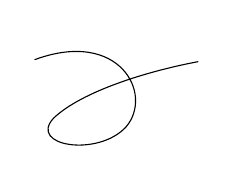
\begin{tikzpicture}[scale=.8]
\draw (-1.1,.65) .. controls (.25,1.15) and (.8,.1) .. (.35,-.42) .. controls (-.1,-.9) and (-1.2,-.72) .. (-.8,-.28) .. controls (-.35,.15) and (.7,.47) .. (1.5,.62);
\end{tikzpicture}},
ou celle-ci:
\figure{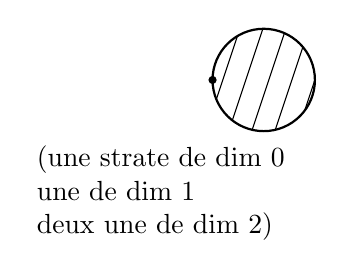
\begin{tikzpicture}[scale=.65]
\begin{scope}\clip (0,0) circle(1);\foreach \x in {-1.2,-.75,-.3,.15,.6}{\draw (\x,-1.2)--(\x+.8,1.2);}\end{scope}
\draw[thick] (0,0) circle(1);\fill (-1,0) circle(.08);
\node[anchor=north east,align=left] at (.6,-1.1) {(une strate de dim 0\\une de dim 1\\\deleted{\unsure{deux}} \inserted{une} de dim 2)};
\end{tikzpicture}}).
Plus précisément encore, on veut ceci:

e) $\forall X_i$, la structure locale autour des $X_i$ \inserted{\unsure{de l'ens.}} des $\overline{X_j}$ tels que $\overline{X_j}\supset X_i$ est \deleted{loc.}

\margin{180}
